Carrier Sense Multiple Access with Enhanced Collision Avoidance (CSMA/ECA)~\cite{CSMA_ECA} achieves less collisions and outperforms CSMA/CA in most typical scenarios. This is done by picking a deterministic backoff after each successful transmission. Its evolution, CSMA/E2CA introduces stickiness in the process in order to shorten the convergence time towards a collision-free state by setting a number of occasions a deterministic backoff is used after each successful transmission.

Stickiness can reduce the convergence time by orders of magnitude when the number of contenders $\eta$ is less or equal than the expectation of the random backoff used in CSMA/CA, $C$. The same constraint is valid for improvements in throughput, as can be appreciated in Figure~\ref{fig:throughput}.

\begin{figure}[htbp]
  \centering
%   \psfrag{psfrag1}[Bc][Bc][0.9]{$\eta$}
  \includegraphics[width=0.7\linewidth, angle = -90]{figures/throughput/throughput.eps}
  \caption{Throughput and how it is affected when $\eta \geq C$
  \label{fig:throughput}}
\end{figure}

In Figure~\ref{fig:throughput}, when $\eta \geq C$ the CSMA/E2CA system is overcrowded with contenders and the collision-free state is compromised. As more contenders are introduced, the system behavior tends to be more like CSMA/CA.

In this work, a fully-distributed version of CSMA/E2CA is presented and the throughput issue when $\eta \geq C$ is assessed using Fair Share.